% Options for packages loaded elsewhere
\PassOptionsToPackage{unicode}{hyperref}
\PassOptionsToPackage{hyphens}{url}
%
\documentclass[
]{article}
\usepackage{amsmath,amssymb}
\usepackage{lmodern}
\usepackage{iftex}
\ifPDFTeX
  \usepackage[T1]{fontenc}
  \usepackage[utf8]{inputenc}
  \usepackage{textcomp} % provide euro and other symbols
\else % if luatex or xetex
  \usepackage{unicode-math}
  \defaultfontfeatures{Scale=MatchLowercase}
  \defaultfontfeatures[\rmfamily]{Ligatures=TeX,Scale=1}
\fi
% Use upquote if available, for straight quotes in verbatim environments
\IfFileExists{upquote.sty}{\usepackage{upquote}}{}
\IfFileExists{microtype.sty}{% use microtype if available
  \usepackage[]{microtype}
  \UseMicrotypeSet[protrusion]{basicmath} % disable protrusion for tt fonts
}{}
\makeatletter
\@ifundefined{KOMAClassName}{% if non-KOMA class
  \IfFileExists{parskip.sty}{%
    \usepackage{parskip}
  }{% else
    \setlength{\parindent}{0pt}
    \setlength{\parskip}{6pt plus 2pt minus 1pt}}
}{% if KOMA class
  \KOMAoptions{parskip=half}}
\makeatother
\usepackage{xcolor}
\usepackage[margin=1in]{geometry}
\usepackage{color}
\usepackage{fancyvrb}
\newcommand{\VerbBar}{|}
\newcommand{\VERB}{\Verb[commandchars=\\\{\}]}
\DefineVerbatimEnvironment{Highlighting}{Verbatim}{commandchars=\\\{\}}
% Add ',fontsize=\small' for more characters per line
\usepackage{framed}
\definecolor{shadecolor}{RGB}{248,248,248}
\newenvironment{Shaded}{\begin{snugshade}}{\end{snugshade}}
\newcommand{\AlertTok}[1]{\textcolor[rgb]{0.94,0.16,0.16}{#1}}
\newcommand{\AnnotationTok}[1]{\textcolor[rgb]{0.56,0.35,0.01}{\textbf{\textit{#1}}}}
\newcommand{\AttributeTok}[1]{\textcolor[rgb]{0.77,0.63,0.00}{#1}}
\newcommand{\BaseNTok}[1]{\textcolor[rgb]{0.00,0.00,0.81}{#1}}
\newcommand{\BuiltInTok}[1]{#1}
\newcommand{\CharTok}[1]{\textcolor[rgb]{0.31,0.60,0.02}{#1}}
\newcommand{\CommentTok}[1]{\textcolor[rgb]{0.56,0.35,0.01}{\textit{#1}}}
\newcommand{\CommentVarTok}[1]{\textcolor[rgb]{0.56,0.35,0.01}{\textbf{\textit{#1}}}}
\newcommand{\ConstantTok}[1]{\textcolor[rgb]{0.00,0.00,0.00}{#1}}
\newcommand{\ControlFlowTok}[1]{\textcolor[rgb]{0.13,0.29,0.53}{\textbf{#1}}}
\newcommand{\DataTypeTok}[1]{\textcolor[rgb]{0.13,0.29,0.53}{#1}}
\newcommand{\DecValTok}[1]{\textcolor[rgb]{0.00,0.00,0.81}{#1}}
\newcommand{\DocumentationTok}[1]{\textcolor[rgb]{0.56,0.35,0.01}{\textbf{\textit{#1}}}}
\newcommand{\ErrorTok}[1]{\textcolor[rgb]{0.64,0.00,0.00}{\textbf{#1}}}
\newcommand{\ExtensionTok}[1]{#1}
\newcommand{\FloatTok}[1]{\textcolor[rgb]{0.00,0.00,0.81}{#1}}
\newcommand{\FunctionTok}[1]{\textcolor[rgb]{0.00,0.00,0.00}{#1}}
\newcommand{\ImportTok}[1]{#1}
\newcommand{\InformationTok}[1]{\textcolor[rgb]{0.56,0.35,0.01}{\textbf{\textit{#1}}}}
\newcommand{\KeywordTok}[1]{\textcolor[rgb]{0.13,0.29,0.53}{\textbf{#1}}}
\newcommand{\NormalTok}[1]{#1}
\newcommand{\OperatorTok}[1]{\textcolor[rgb]{0.81,0.36,0.00}{\textbf{#1}}}
\newcommand{\OtherTok}[1]{\textcolor[rgb]{0.56,0.35,0.01}{#1}}
\newcommand{\PreprocessorTok}[1]{\textcolor[rgb]{0.56,0.35,0.01}{\textit{#1}}}
\newcommand{\RegionMarkerTok}[1]{#1}
\newcommand{\SpecialCharTok}[1]{\textcolor[rgb]{0.00,0.00,0.00}{#1}}
\newcommand{\SpecialStringTok}[1]{\textcolor[rgb]{0.31,0.60,0.02}{#1}}
\newcommand{\StringTok}[1]{\textcolor[rgb]{0.31,0.60,0.02}{#1}}
\newcommand{\VariableTok}[1]{\textcolor[rgb]{0.00,0.00,0.00}{#1}}
\newcommand{\VerbatimStringTok}[1]{\textcolor[rgb]{0.31,0.60,0.02}{#1}}
\newcommand{\WarningTok}[1]{\textcolor[rgb]{0.56,0.35,0.01}{\textbf{\textit{#1}}}}
\usepackage{graphicx}
\makeatletter
\def\maxwidth{\ifdim\Gin@nat@width>\linewidth\linewidth\else\Gin@nat@width\fi}
\def\maxheight{\ifdim\Gin@nat@height>\textheight\textheight\else\Gin@nat@height\fi}
\makeatother
% Scale images if necessary, so that they will not overflow the page
% margins by default, and it is still possible to overwrite the defaults
% using explicit options in \includegraphics[width, height, ...]{}
\setkeys{Gin}{width=\maxwidth,height=\maxheight,keepaspectratio}
% Set default figure placement to htbp
\makeatletter
\def\fps@figure{htbp}
\makeatother
\setlength{\emergencystretch}{3em} % prevent overfull lines
\providecommand{\tightlist}{%
  \setlength{\itemsep}{0pt}\setlength{\parskip}{0pt}}
\setcounter{secnumdepth}{-\maxdimen} % remove section numbering
\usepackage{booktabs}
\usepackage{longtable}
\usepackage{array}
\usepackage{multirow}
\usepackage{wrapfig}
\usepackage{float}
\usepackage{colortbl}
\usepackage{pdflscape}
\usepackage{tabu}
\usepackage{threeparttable}
\usepackage{threeparttablex}
\usepackage[normalem]{ulem}
\usepackage{makecell}
\usepackage{xcolor}
\ifLuaTeX
  \usepackage{selnolig}  % disable illegal ligatures
\fi
\IfFileExists{bookmark.sty}{\usepackage{bookmark}}{\usepackage{hyperref}}
\IfFileExists{xurl.sty}{\usepackage{xurl}}{} % add URL line breaks if available
\urlstyle{same} % disable monospaced font for URLs
\hypersetup{
  pdftitle={DATA 606 Fall 2022 - Final Exam},
  pdfauthor={Alex Khaykin},
  hidelinks,
  pdfcreator={LaTeX via pandoc}}

\title{DATA 606 Fall 2022 - Final Exam}
\author{Alex Khaykin}
\date{}

\begin{document}
\maketitle

\begin{verbatim}
## Warning: package 'tidyverse' was built under R version 4.2.2
\end{verbatim}

\begin{verbatim}
## -- Attaching packages --------------------------------------- tidyverse 1.3.2 --
## v ggplot2 3.3.6     v purrr   0.3.4
## v tibble  3.1.8     v dplyr   1.0.9
## v tidyr   1.2.0     v stringr 1.4.1
## v readr   2.1.2     v forcats 0.5.2
## -- Conflicts ------------------------------------------ tidyverse_conflicts() --
## x dplyr::filter() masks stats::filter()
## x dplyr::lag()    masks stats::lag()
\end{verbatim}

\hypertarget{part-i}{%
\section{Part I}\label{part-i}}

Please put the answers for Part I next to the question number (please
enter only the letter options; 4 points each):

\begin{enumerate}
\def\labelenumi{\arabic{enumi}.}
\item
  \begin{enumerate}
  \def\labelenumii{\Alph{enumii})}
  \setcounter{enumii}{1}
  \tightlist
  \item
    3.01 ± 2.977(0.534/ sqrt(15)
  \end{enumerate}
\item
  \begin{enumerate}
  \def\labelenumii{\Alph{enumii})}
  \tightlist
  \item
    Deciding that the absorption rates are different, when in fact they
    are not.
  \end{enumerate}
\item
  \begin{enumerate}
  \def\labelenumii{\Alph{enumii})}
  \setcounter{enumii}{3}
  \tightlist
  \item
    0.070
  \end{enumerate}
\item
  \begin{enumerate}
  \def\labelenumii{\Alph{enumii})}
  \setcounter{enumii}{1}
  \tightlist
  \item
    2-proportion z-test
  \end{enumerate}
\item
  \begin{enumerate}
  \def\labelenumii{\Alph{enumii})}
  \setcounter{enumii}{1}
  \tightlist
  \item
    II only
  \end{enumerate}
\item
  \begin{enumerate}
  \def\labelenumii{\Alph{enumii})}
  \setcounter{enumii}{4}
  \tightlist
  \item
    1600
  \end{enumerate}
\item
  \begin{enumerate}
  \def\labelenumii{\Alph{enumii})}
  \setcounter{enumii}{3}
  \tightlist
  \item
    the probability of the observed statistic given that the null
    hypothesis is true.
  \end{enumerate}
\item
  \begin{enumerate}
  \def\labelenumii{\Alph{enumii})}
  \setcounter{enumii}{3}
  \tightlist
  \item
    They fail to reject H0 , making a Type I error
  \end{enumerate}
\item
  \begin{enumerate}
  \def\labelenumii{\Alph{enumii})}
  \setcounter{enumii}{1}
  \tightlist
  \item
    there is a strong linear relationship between the two variables
  \end{enumerate}
\item
  \begin{enumerate}
  \def\labelenumii{\Alph{enumii})}
  \setcounter{enumii}{2}
  \tightlist
  \item
    the expected y value when x is zero
  \end{enumerate}
\end{enumerate}

\hypertarget{part-ii}{%
\section{Part II}\label{part-ii}}

Consider the three datasets, each with two columns (x and y), provided
below. Be sure to replace the \texttt{NA} with your answer for each part
(e.g.~assign the mean of \texttt{x} for \texttt{data1} to the
\texttt{data1.x.mean} variable). When you Knit your answer document, a
table will be generated with all the answers.

For each column, calculate (to four decimal places):

\hypertarget{a.-the-mean-for-x-and-y-separately-5-pt.}{%
\paragraph{a. The mean (for x and y separately; 5
pt).}\label{a.-the-mean-for-x-and-y-separately-5-pt.}}

\begin{Shaded}
\begin{Highlighting}[]
\NormalTok{data1.x.mean }\OtherTok{\textless{}{-}} \FunctionTok{round}\NormalTok{(}\FunctionTok{mean}\NormalTok{(data1}\SpecialCharTok{$}\NormalTok{x), }\AttributeTok{digits =} \DecValTok{4}\NormalTok{)}
\NormalTok{data1.y.mean }\OtherTok{\textless{}{-}} \FunctionTok{round}\NormalTok{(}\FunctionTok{mean}\NormalTok{(data1}\SpecialCharTok{$}\NormalTok{y), }\AttributeTok{digits =} \DecValTok{4}\NormalTok{)}
\NormalTok{data2.x.mean }\OtherTok{\textless{}{-}} \FunctionTok{round}\NormalTok{(}\FunctionTok{mean}\NormalTok{(data2}\SpecialCharTok{$}\NormalTok{x), }\AttributeTok{digits =} \DecValTok{4}\NormalTok{)}
\NormalTok{data2.y.mean }\OtherTok{\textless{}{-}} \FunctionTok{round}\NormalTok{(}\FunctionTok{mean}\NormalTok{(data2}\SpecialCharTok{$}\NormalTok{y), }\AttributeTok{digits =} \DecValTok{4}\NormalTok{)}
\NormalTok{data3.x.mean }\OtherTok{\textless{}{-}} \FunctionTok{round}\NormalTok{(}\FunctionTok{mean}\NormalTok{(data3}\SpecialCharTok{$}\NormalTok{x), }\AttributeTok{digits =} \DecValTok{4}\NormalTok{)}
\NormalTok{data3.y.mean }\OtherTok{\textless{}{-}} \FunctionTok{round}\NormalTok{(}\FunctionTok{mean}\NormalTok{(data3}\SpecialCharTok{$}\NormalTok{y), }\AttributeTok{digits =} \DecValTok{4}\NormalTok{)}
\end{Highlighting}
\end{Shaded}

\hypertarget{b.-the-median-for-x-and-y-separately-5-pt.}{%
\paragraph{b. The median (for x and y separately; 5
pt).}\label{b.-the-median-for-x-and-y-separately-5-pt.}}

\begin{Shaded}
\begin{Highlighting}[]
\NormalTok{data1.x.median }\OtherTok{\textless{}{-}} \FunctionTok{round}\NormalTok{(}\FunctionTok{median}\NormalTok{(data1}\SpecialCharTok{$}\NormalTok{x), }\AttributeTok{digits =} \DecValTok{4}\NormalTok{)}
\NormalTok{data1.y.median }\OtherTok{\textless{}{-}} \FunctionTok{round}\NormalTok{(}\FunctionTok{median}\NormalTok{(data1}\SpecialCharTok{$}\NormalTok{y), }\AttributeTok{digits =} \DecValTok{4}\NormalTok{)}
\NormalTok{data2.x.median }\OtherTok{\textless{}{-}} \FunctionTok{round}\NormalTok{(}\FunctionTok{median}\NormalTok{(data2}\SpecialCharTok{$}\NormalTok{x), }\AttributeTok{digits =} \DecValTok{4}\NormalTok{)}
\NormalTok{data2.y.median }\OtherTok{\textless{}{-}} \FunctionTok{round}\NormalTok{(}\FunctionTok{median}\NormalTok{(data2}\SpecialCharTok{$}\NormalTok{y), }\AttributeTok{digits =} \DecValTok{4}\NormalTok{)}
\NormalTok{data3.x.median }\OtherTok{\textless{}{-}} \FunctionTok{round}\NormalTok{(}\FunctionTok{median}\NormalTok{(data3}\SpecialCharTok{$}\NormalTok{x), }\AttributeTok{digits =} \DecValTok{4}\NormalTok{)}
\NormalTok{data3.y.median }\OtherTok{\textless{}{-}} \FunctionTok{round}\NormalTok{(}\FunctionTok{median}\NormalTok{(data3}\SpecialCharTok{$}\NormalTok{y), }\AttributeTok{digits =} \DecValTok{4}\NormalTok{)}
\end{Highlighting}
\end{Shaded}

\hypertarget{c.-the-standard-deviation-for-x-and-y-separately-5-pt.}{%
\paragraph{c.~The standard deviation (for x and y separately; 5
pt).}\label{c.-the-standard-deviation-for-x-and-y-separately-5-pt.}}

\begin{Shaded}
\begin{Highlighting}[]
\NormalTok{data1.x.sd }\OtherTok{\textless{}{-}} \FunctionTok{round}\NormalTok{(}\FunctionTok{sd}\NormalTok{(data1}\SpecialCharTok{$}\NormalTok{x), }\AttributeTok{digits =} \DecValTok{4}\NormalTok{)}
\NormalTok{data1.y.sd }\OtherTok{\textless{}{-}} \FunctionTok{round}\NormalTok{(}\FunctionTok{sd}\NormalTok{(data1}\SpecialCharTok{$}\NormalTok{y), }\AttributeTok{digits =} \DecValTok{4}\NormalTok{)}
\NormalTok{data2.x.sd }\OtherTok{\textless{}{-}} \FunctionTok{round}\NormalTok{(}\FunctionTok{sd}\NormalTok{(data2}\SpecialCharTok{$}\NormalTok{x), }\AttributeTok{digits =} \DecValTok{4}\NormalTok{)}
\NormalTok{data2.y.sd }\OtherTok{\textless{}{-}} \FunctionTok{round}\NormalTok{(}\FunctionTok{sd}\NormalTok{(data2}\SpecialCharTok{$}\NormalTok{y), }\AttributeTok{digits =} \DecValTok{4}\NormalTok{)}
\NormalTok{data3.x.sd }\OtherTok{\textless{}{-}} \FunctionTok{round}\NormalTok{(}\FunctionTok{sd}\NormalTok{(data3}\SpecialCharTok{$}\NormalTok{x), }\AttributeTok{digits =} \DecValTok{4}\NormalTok{)}
\NormalTok{data3.y.sd }\OtherTok{\textless{}{-}} \FunctionTok{round}\NormalTok{(}\FunctionTok{sd}\NormalTok{(data3}\SpecialCharTok{$}\NormalTok{y), }\AttributeTok{digits =} \DecValTok{4}\NormalTok{)}
\end{Highlighting}
\end{Shaded}

\hypertarget{for-each-x-and-y-pair-calculate-also-to-two-decimal-places}{%
\paragraph{For each x and y pair, calculate (also to two decimal
places):}\label{for-each-x-and-y-pair-calculate-also-to-two-decimal-places}}

\hypertarget{d.-the-correlation-5-pt.}{%
\paragraph{d.~The correlation (5 pt).}\label{d.-the-correlation-5-pt.}}

\begin{Shaded}
\begin{Highlighting}[]
\FunctionTok{options}\NormalTok{(}\AttributeTok{digits =} \DecValTok{2}\NormalTok{)}
\NormalTok{data1.correlation }\OtherTok{\textless{}{-}} \FunctionTok{round}\NormalTok{(}\FunctionTok{cor}\NormalTok{(data1}\SpecialCharTok{$}\NormalTok{x, data1}\SpecialCharTok{$}\NormalTok{y), }\AttributeTok{digits =} \DecValTok{2}\NormalTok{)}
\NormalTok{data2.correlation }\OtherTok{\textless{}{-}} \FunctionTok{round}\NormalTok{(}\FunctionTok{cor}\NormalTok{(data2}\SpecialCharTok{$}\NormalTok{x, data2}\SpecialCharTok{$}\NormalTok{y), }\AttributeTok{digits =} \DecValTok{2}\NormalTok{)}
\NormalTok{data3.correlation }\OtherTok{\textless{}{-}} \FunctionTok{round}\NormalTok{(}\FunctionTok{cor}\NormalTok{(data3}\SpecialCharTok{$}\NormalTok{x, data3}\SpecialCharTok{$}\NormalTok{y), }\AttributeTok{digits =} \DecValTok{2}\NormalTok{)}
\end{Highlighting}
\end{Shaded}

\hypertarget{e.-linear-regression-equation-5-points.}{%
\paragraph{e. Linear regression equation (5
points).}\label{e.-linear-regression-equation-5-points.}}

\begin{Shaded}
\begin{Highlighting}[]
\NormalTok{data1.slope }\OtherTok{\textless{}{-}} \FunctionTok{round}\NormalTok{(}\FunctionTok{coef}\NormalTok{(}\FunctionTok{lm}\NormalTok{(y }\SpecialCharTok{\textasciitilde{}}\NormalTok{x, }\AttributeTok{data =}\NormalTok{ data1))[}\DecValTok{2}\NormalTok{], }\AttributeTok{digits =} \DecValTok{2}\NormalTok{)}
\NormalTok{data2.slope }\OtherTok{\textless{}{-}} \FunctionTok{round}\NormalTok{(}\FunctionTok{coef}\NormalTok{(}\FunctionTok{lm}\NormalTok{(y }\SpecialCharTok{\textasciitilde{}}\NormalTok{x, }\AttributeTok{data =}\NormalTok{ data2))[}\DecValTok{2}\NormalTok{], }\AttributeTok{digits =} \DecValTok{2}\NormalTok{)}
\NormalTok{data3.slope }\OtherTok{\textless{}{-}} \FunctionTok{round}\NormalTok{(}\FunctionTok{coef}\NormalTok{(}\FunctionTok{lm}\NormalTok{(y }\SpecialCharTok{\textasciitilde{}}\NormalTok{x, }\AttributeTok{data =}\NormalTok{ data3))[}\DecValTok{2}\NormalTok{], }\AttributeTok{digits =} \DecValTok{2}\NormalTok{)}

\NormalTok{data1.intercept }\OtherTok{\textless{}{-}} \FunctionTok{round}\NormalTok{(}\FunctionTok{coef}\NormalTok{(}\FunctionTok{lm}\NormalTok{(y }\SpecialCharTok{\textasciitilde{}}\NormalTok{x, }\AttributeTok{data =}\NormalTok{ data1))[}\DecValTok{1}\NormalTok{], }\AttributeTok{digits =} \DecValTok{2}\NormalTok{)}
\NormalTok{data2.intercept }\OtherTok{\textless{}{-}} \FunctionTok{round}\NormalTok{(}\FunctionTok{coef}\NormalTok{(}\FunctionTok{lm}\NormalTok{(y }\SpecialCharTok{\textasciitilde{}}\NormalTok{x, }\AttributeTok{data =}\NormalTok{ data2))[}\DecValTok{1}\NormalTok{], }\AttributeTok{digits =} \DecValTok{2}\NormalTok{)}
\NormalTok{data3.intercept }\OtherTok{\textless{}{-}} \FunctionTok{round}\NormalTok{(}\FunctionTok{coef}\NormalTok{(}\FunctionTok{lm}\NormalTok{(y }\SpecialCharTok{\textasciitilde{}}\NormalTok{x, }\AttributeTok{data =}\NormalTok{ data3))[}\DecValTok{1}\NormalTok{], }\AttributeTok{digits =} \DecValTok{2}\NormalTok{)}
\end{Highlighting}
\end{Shaded}

\hypertarget{f.-r-squared-5-points.}{%
\paragraph{f.~R-Squared (5 points).}\label{f.-r-squared-5-points.}}

\begin{Shaded}
\begin{Highlighting}[]
\NormalTok{data1.rsquared }\OtherTok{\textless{}{-}} \FunctionTok{round}\NormalTok{(}\FunctionTok{summary}\NormalTok{(}\FunctionTok{lm}\NormalTok{(y }\SpecialCharTok{\textasciitilde{}}\NormalTok{ x, }\AttributeTok{data =}\NormalTok{ data1))}\SpecialCharTok{$}\NormalTok{r.squared, }\AttributeTok{digits =} \DecValTok{2}\NormalTok{)}
\NormalTok{data2.rsquared }\OtherTok{\textless{}{-}} \FunctionTok{round}\NormalTok{(}\FunctionTok{summary}\NormalTok{(}\FunctionTok{lm}\NormalTok{(y }\SpecialCharTok{\textasciitilde{}}\NormalTok{ x, }\AttributeTok{data =}\NormalTok{ data2))}\SpecialCharTok{$}\NormalTok{r.squared, }\AttributeTok{digits =} \DecValTok{2}\NormalTok{)}
\NormalTok{data3.rsquared }\OtherTok{\textless{}{-}} \FunctionTok{round}\NormalTok{(}\FunctionTok{summary}\NormalTok{(}\FunctionTok{lm}\NormalTok{(y }\SpecialCharTok{\textasciitilde{}}\NormalTok{ x, }\AttributeTok{data =}\NormalTok{ data3))}\SpecialCharTok{$}\NormalTok{r.squared, }\AttributeTok{digits =} \DecValTok{2}\NormalTok{)}
\end{Highlighting}
\end{Shaded}

Summary Table

\begin{verbatim}
## Warning: package 'kableExtra' was built under R version 4.2.2
\end{verbatim}

\begin{verbatim}
## 
## Attaching package: 'kableExtra'
\end{verbatim}

\begin{verbatim}
## The following object is masked from 'package:dplyr':
## 
##     group_rows
\end{verbatim}

\begin{tabular}{l|>{\raggedleft\arraybackslash}p{.5in}|>{\raggedleft\arraybackslash}p{.5in}|>{\raggedleft\arraybackslash}p{.5in}|>{\raggedleft\arraybackslash}p{.5in}|>{\raggedleft\arraybackslash}p{.5in}|>{\raggedleft\arraybackslash}p{.5in}}
\hline
\multicolumn{1}{c|}{ } & \multicolumn{2}{c|}{Data 1} & \multicolumn{2}{c|}{Data 2} & \multicolumn{2}{c}{Data 3} \\
\cline{2-3} \cline{4-5} \cline{6-7}
  & x & y & x & y & x & y\\
\hline
Mean & 54.2633 & 47.8323 & 54.2678 & 47.8359 & 54.2661 & 47.8347\\
\hline
Median & 53.3333 & 46.0256 & 53.1352 & 46.4013 & 53.3403 & 47.5353\\
\hline
SD & 16.7651 & 26.9354 & 16.7668 & 26.9361 & 16.7698 & 26.9397\\
\hline
r & -0.0600 &  & -0.0700 &  & -0.0600 & \\
\hline
Intercept & 53.4500 &  & 53.8500 &  & 53.4300 & \\
\hline
Slope & -0.1000 &  & -0.1100 &  & -0.1000 & \\
\hline
R-Squared & 0.0000 &  & 0.0000 &  & 0.0000 & \\
\hline
\end{tabular}

\hypertarget{g.-for-each-pair-is-it-appropriate-to-estimate-a-linear-regression-model-why-or-why-not-be-specific-as-to-why-for-each-pair-and-include-appropriate-plots-15-points}{%
\paragraph{g. For each pair, is it appropriate to estimate a linear
regression model? Why or why not? Be specific as to why for each pair
and include appropriate plots! (15
points)}\label{g.-for-each-pair-is-it-appropriate-to-estimate-a-linear-regression-model-why-or-why-not-be-specific-as-to-why-for-each-pair-and-include-appropriate-plots-15-points}}

\#Answer It is not appropriated to

\begin{Shaded}
\begin{Highlighting}[]
\FunctionTok{ggplot}\NormalTok{(data1, }\FunctionTok{aes}\NormalTok{(}\AttributeTok{x =}\NormalTok{ x, }\AttributeTok{y =}\NormalTok{ y)) }\SpecialCharTok{+}
  \FunctionTok{geom\_point}\NormalTok{() }\SpecialCharTok{+}
  \FunctionTok{stat\_smooth}\NormalTok{(}\AttributeTok{formula =} \StringTok{"y \textasciitilde{} x"}\NormalTok{, }\AttributeTok{se =} \ConstantTok{FALSE}\NormalTok{, }\AttributeTok{method =} \StringTok{"lm"}\NormalTok{)}
\end{Highlighting}
\end{Shaded}

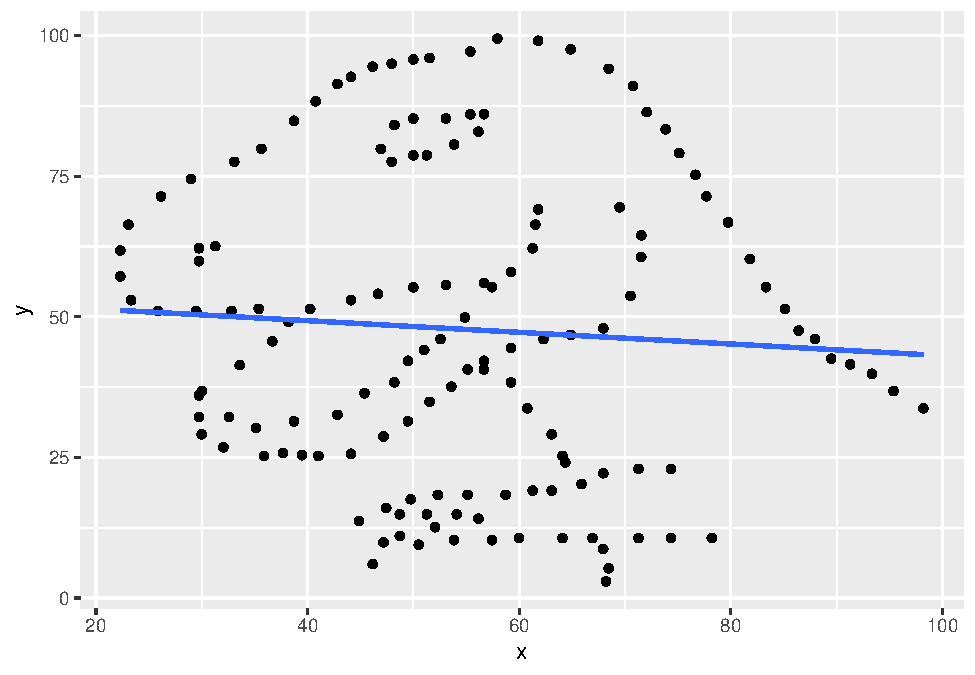
\includegraphics{Final_Exam_Answers_in_Progress_files/figure-latex/unnamed-chunk-11-1.pdf}

\begin{Shaded}
\begin{Highlighting}[]
\FunctionTok{ggplot}\NormalTok{(data2, }\FunctionTok{aes}\NormalTok{(}\AttributeTok{x =}\NormalTok{ x, }\AttributeTok{y =}\NormalTok{ y)) }\SpecialCharTok{+}
  \FunctionTok{geom\_point}\NormalTok{() }\SpecialCharTok{+}
  \FunctionTok{stat\_smooth}\NormalTok{(}\AttributeTok{formula =} \StringTok{"y \textasciitilde{} x"}\NormalTok{, }\AttributeTok{se =} \ConstantTok{FALSE}\NormalTok{, }\AttributeTok{method =} \StringTok{"lm"}\NormalTok{)}
\end{Highlighting}
\end{Shaded}

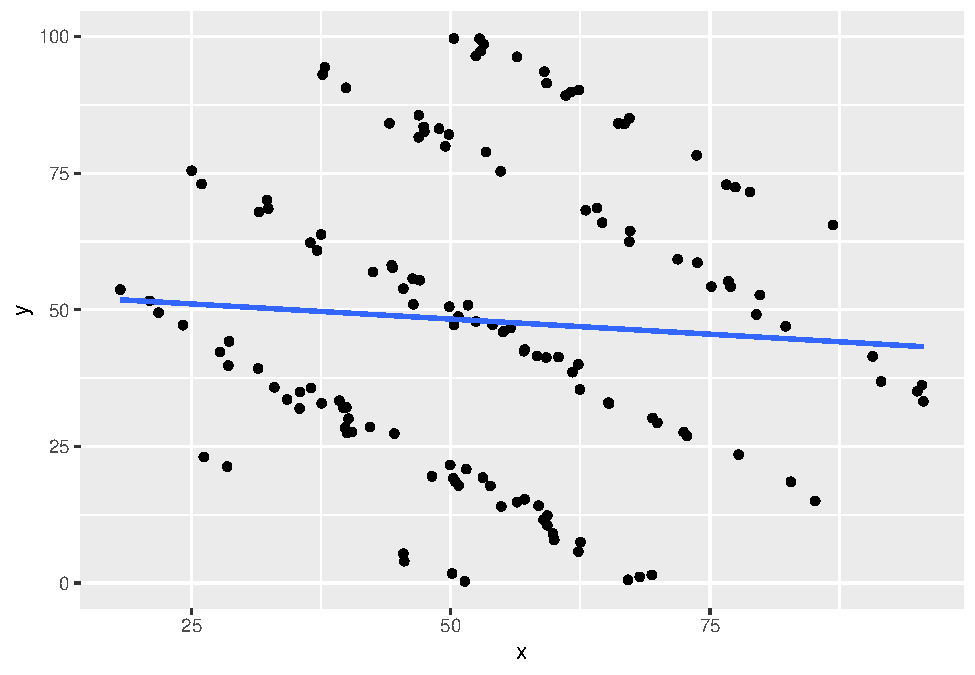
\includegraphics{Final_Exam_Answers_in_Progress_files/figure-latex/unnamed-chunk-11-2.pdf}

\begin{Shaded}
\begin{Highlighting}[]
\FunctionTok{ggplot}\NormalTok{(data3, }\FunctionTok{aes}\NormalTok{(}\AttributeTok{x =}\NormalTok{ x, }\AttributeTok{y =}\NormalTok{ y)) }\SpecialCharTok{+}
  \FunctionTok{geom\_point}\NormalTok{() }\SpecialCharTok{+}
  \FunctionTok{stat\_smooth}\NormalTok{(}\AttributeTok{formula =} \StringTok{"y \textasciitilde{} x"}\NormalTok{, }\AttributeTok{se =} \ConstantTok{FALSE}\NormalTok{, }\AttributeTok{method =} \StringTok{"lm"}\NormalTok{)}
\end{Highlighting}
\end{Shaded}

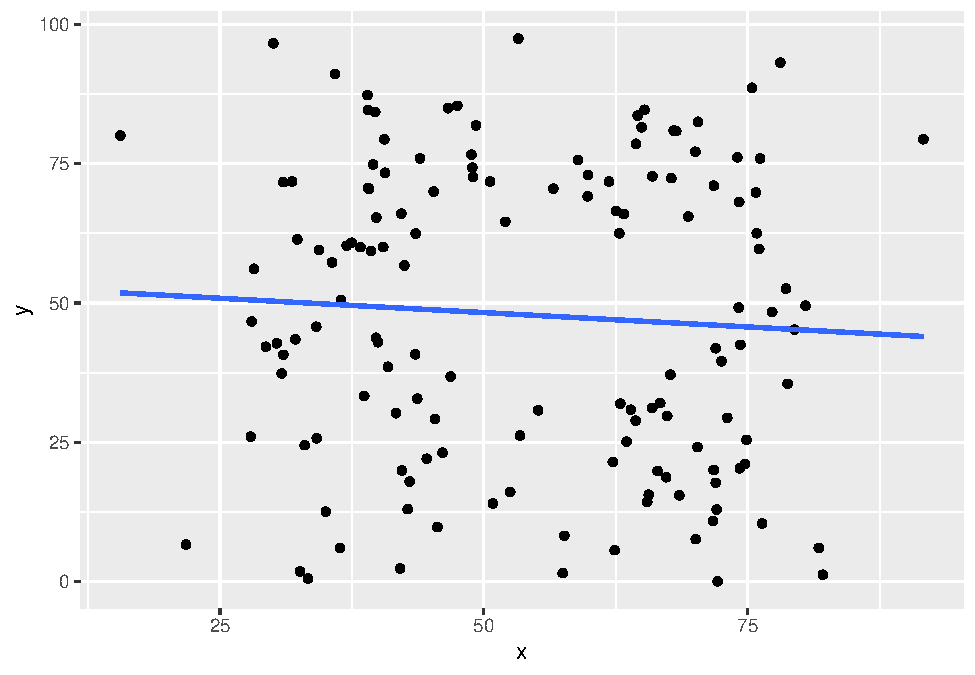
\includegraphics{Final_Exam_Answers_in_Progress_files/figure-latex/unnamed-chunk-11-3.pdf}

\hypertarget{h.-explain-why-it-is-important-to-include-appropriate-visualizations-when-analyzing-data.-include-any-visualizations-you-create.-15-points}{%
\paragraph{h. Explain why it is important to include appropriate
visualizations when analyzing data. Include any visualization(s) you
create. (15
points)}\label{h.-explain-why-it-is-important-to-include-appropriate-visualizations-when-analyzing-data.-include-any-visualizations-you-create.-15-points}}

\end{document}
